\documentclass{beamer}[10]

\usepackage{graphicx}
\usepackage{xcolor}
\usepackage{tabto}
%\usepackage{beamerthemesplit}
\usepackage{tikz}
\usepackage{cancel}
\usepackage{verbatim}
\usepackage{fancybox}
\usepackage{enumerate}
\usepackage{amsmath,amssymb,amsthm,textcomp,mathtools}
\usepackage[super]{nth}
\usepackage[amssymb]{SIunits}
\usepackage{booktabs}
\usepackage{cancel}
\usepackage{bm}
\usepackage[utf8]{inputenc}
\usepackage{tabularx}
\usepackage{ragged2e}
\newcolumntype{Y}{ >{\RaggedRight\arraybackslash}X}
\usetikzlibrary{arrows,shapes}
\newcommand\T{\rule{0pt}{2.6ex}}
\newcommand\B{\rule[-1.2ex]{0pt}{0pt}}
\definecolor{UUcrimson}{RGB}{204,0,0}
\mode<presentation>
{ \usetheme{default}
  \usecolortheme[named=UUcrimson]{structure}
  \useinnertheme{circles}
  \setbeamercovered{transparent}
  \setbeamertemplate{blocks}[rounded]
  \usefonttheme[onlymath]{serif}
  \setbeamertemplate{navigation symbols}{}
  \setbeamertemplate{footline}[page number]
  \setbeamertemplate{navigation symbols}{}
  \setbeamercolor{section in toc}{fg=black,bg=white}
  \setbeamercolor{alerted text}{fg=UUcrimson!80!gray}
  \setbeamercolor*{palette primary}{fg=white,bg=UUcrimson}
  \setbeamercolor*{palette secondary}{fg=UUcrimson!70!black,bg=gray!15!white}
  \setbeamercolor*{palette tertiary}{bg=UUcrimson!80!black,fg=gray!10!white}
  \setbeamercolor*{palette quaternary}{fg=UUcrimson,bg=gray!5!white}
  \setbeamercolor*{palette sidebar primary}{fg=UUcrimson!10!black}
  \setbeamercolor*{palette sidebar secondary}{fg=white}
  \setbeamercolor*{palette sidebar tertiary}{fg=UUcrimson!50!black}
  \setbeamercolor*{palette sidebar quaternary}{fg=gray!10!white}
  \setbeamercolor{titlelike}{parent=palette primary,fg=white}
  \setbeamercolor{frametitle}{bg=UUcrimson}
  \setbeamercolor{frametitle right}{bg=UUcrimson}
  \setbeamercolor*{separation line}{}
  \setbeamercolor*{fine separation line}{}
}

\usetikzlibrary{backgrounds}
\makeatletter
\tikzstyle{every picture}+=[remember picture]
\tikzset{%
  fancy quotes/.style={
    text width=\fq@width pt,
    align=justify,
    inner sep=1em,
    anchor=north west,
    minimum width=\linewidth,
    font=\itshape
  },
  fancy quotes width/.initial={.8\linewidth},
  fancy quotes marks/.style={
    scale=8,
    text=white,
    inner sep=0pt,
  },
  fancy quotes opening/.style={
    fancy quotes marks,
  },
  fancy quotes closing/.style={
    fancy quotes marks,
  },
  fancy quotes background/.style={
    show background rectangle,
    inner frame xsep=0pt,
    background rectangle/.style={
      fill=gray!25,
      rounded corners,
    },
  }
}
\newenvironment{fancyquotes}[1][]{%
\noindent
\tikzpicture[fancy quotes background]
\node[fancy quotes opening,anchor=north west] (fq@ul) at (0,0) {``};
\tikz@scan@one@point\pgfutil@firstofone(fq@ul.east)
\pgfmathsetmacro{\fq@width}{\linewidth - 2*\pgf@x}
\node[fancy quotes,#1] (fq@txt) at (fq@ul.north west) \bgroup}
{\egroup;
\node[overlay,fancy quotes closing,anchor=east] at (fq@txt.south east) {''};
\endtikzpicture}
\makeatother


\usetikzlibrary{backgrounds}
\makeatletter
\tikzstyle{every picture}+=[remember picture]
\tikzset{%
  fancy defs/.style={
    text width=\fq@width pt,
    align=justify,
    inner sep=0.25em,
    anchor=north west,
    minimum width=\linewidth,
    font=\itshape
  },
  fancy defs width/.initial={.8\linewidth},
  fancy defs marks/.style={
    scale=8,
    text=white,
    inner sep=0pt,
  },
  fancy defs opening/.style={
    fancy defs marks,
  },
  fancy defs closing/.style={
    fancy defs marks,
  },
  fancy defs background/.style={
    show background rectangle,
    inner frame xsep=0pt,
    background rectangle/.style={
      fill=gray!25,
      rounded corners,
    },
  }
}
\newenvironment{fancydefs}[1][]{%
\noindent
\tikzpicture[fancy defs background]
\node[fancy defs opening,anchor=north west] (fq@ul) at (0,0) {};
\tikz@scan@one@point\pgfutil@firstofone(fq@ul.east)
\pgfmathsetmacro{\fq@width}{\linewidth - 2*\pgf@x}
\node[fancy defs,#1] (fq@txt) at (fq@ul.north west) \bgroup}
{\egroup;
\node[overlay,fancy defs closing,anchor=east] at (fq@txt.south east) {};
\endtikzpicture}
\makeatother
\usepackage{scalerel}[2014/03/10]
\usepackage{stackengine}
\usepackage{empheq}
\newcommand*\widefbox[1]{\fbox{\hspace{0.5em}#1\hspace{0.5em}}}

\newcommand\reallywidetilde[1]{\ThisStyle{%
  \setbox0=\hbox{$\SavedStyle#1$}%
  \stackengine{-.1\LMpt}{$\SavedStyle#1$}{%
    \stretchto{\scaleto{\SavedStyle\mkern.2mu\sim}{.5467\wd0}}{.4\ht0}%
%    .2mu is the kern imbalance when clipping white space
%    .5467++++ is \ht/[kerned \wd] aspect ratio for \sim glyph
  }{O}{c}{F}{T}{S}%
}}
\usepackage{media9}

\logo{
\includegraphics[width=0.75cm]{logo.jpg}}
\author[Gibbs]{Dr. Jeremy A. Gibbs}
\institute{Department of Mechanical Engineering\\University of Utah}
\date{Spring 2017}
\title{Environmental Fluid Dynamics: Lecture 6}
% colors
\definecolor{colororange}{HTML}{E65100} % orange
\definecolor{colordgray}{HTML}{795548} % dark gray for note
\definecolor{colorhgray}{HTML}{212121} % heavy dark gray for normal text
\definecolor{colorgreen}{HTML}{009688} % green
\definecolor{colorwhite}{HTML}{FFFFFF} % background white
\definecolor{colorlgray}{HTML}{F5F3EE} % background light gray
\definecolor{colorblue}{HTML}{0277BB} % blue
\definecolor{colorred}{HTML}{CC0000} % red
\newcommand{\fontsizeone}{1.9em}
\setbeamertemplate{caption}{\raggedright\insertcaption\par}
\newcommand{\framecard}[2][colorgreen]{
  {\setbeamercolor{background canvas}{bg=#1}
    \begin{frame}[plain]
    \vfill
    \begin{center}
     {#2}
    \end{center}
    \vfill
    \end{frame}
  }
}
\begin{document}

%----------------------------------------------------------------------------------------
%	TITLE & TOC SLIDES
%----------------------------------------------------------------------------------------

\begin{frame} 
  \titlepage
\end{frame}

%------------------------------------------------

\begin{frame}
\frametitle{Overview}
\tableofcontents
\end{frame}

%------------------------------------------------
\section{Atmospheric Thermodynamics: Water Vapor} %
%------------------------------------------------
\framecard[colorred]{{\color{white}\Huge Atmospheric Thermodynamics:\\~\\Water Vapor}}
%------------------------------------------------
\subsection{Moisture Parameters}
%------------------------------------------------

\begin{frame}{Atmospheric Thermodynamics: Water Vapor}
\begin{itemize}
	\item So far we have discussed water vapor in the air through its vapor pressure $e$
	\item We included its effects on density through the virtual temperature correction
	\item There are many ways in which to describe the amount of water vapor present in the atmosphere - so we will discuss various moisture paramters
	\item What happens when water vapor condenses? We will cover that, too.
\end{itemize}
\end{frame}

%------------------------------------------------

\begin{frame}{Moisture Parameters: Latent Heat}
\textbf{Latent Heat of Vaporization/Evaporation}
\begin{fancydefs}
	The heat required by a unit mass of material to convert it from the liquid to gas phase without a change in temperature
\end{fancydefs}

\begin{itemize}
	\item At 1 atm and $100\ \celsius$ (boiling point of water), $L_v = 2.25\times10^6\ \joule\ \kilo\reciprocal\gram$
	\item The Latent Heat of Condensation has the same value, but heat is released when changing from vapor to liquid
\end{itemize}
\end{frame}

%------------------------------------------------

\begin{frame}{Moisture Parameters: Mixing Ratio}
\textbf{Mixing Ratio}
\begin{fancydefs}
	The amount of water vapor in a volume of air expressed as the ratio of the mass of water vapor $m_v$ to the mass of dry air $m_d$
	$$r \equiv \frac{m_v}{m_d}$$
\end{fancydefs}

\begin{itemize}
	\item Usually expressed as [$\gram_v / \kilo\gram_d$]
	\item Dimensionless for numerical computations [$\kilo\gram_v / \kilo\gram_d$]
	\item Ranges from a few $\gram\ \kilo\reciprocal\gram$ in midlatitudes to $20\ \gram/\kilo\reciprocal\gram$ in the tropics
	\item In the absence of condensation/evaporation, an air parcel's $r$ is constant (conserved)
\end{itemize}
\end{frame}


%------------------------------------------------

\begin{frame}{Moisture Parameters: Mixing Ratio}
\begin{itemize}
	\item We can relate mixing ratio $r$ to $T_v$
	\item Let's recall the notion of partial pressures. The partial pressure of a gas is proportional to the number of moles of that gas present in the mixture
	\begin{align*}
	e &= \cfrac{n_v}{n_d + n_v}p = \cfrac{\cfrac{m_v}{M_w}}{\cfrac{m_d}{M_d} + \cfrac{m_v}{M_w}}p = \cfrac{m_v}{\cfrac{m_dM_w}{M_d} + \cfrac{m_vM_w}{M_w}}p = \cfrac{\cfrac{m_v}{m_d}}{\epsilon\cfrac{m_d}{m_d} + \cfrac{m_v}{m_d}}p\\
	\Aboxed{e&= \frac{r}{r+\epsilon}p}
	\end{align*}
	where, recall, $\epsilon = R_d/R_v = M_w/M_d = 0.622$
\end{itemize}
\end{frame}

%------------------------------------------------

\begin{frame}{Moisture Parameters: Mixing Ratio}
$$e= \frac{r}{r+\epsilon}p$$
\begin{itemize}
	\item Recall from Lecture 4 that
	$$T_v \equiv \frac{T}{1 - \frac{e}{p}(1-\epsilon)}$$
	\item Replace $e/p$ with the expression derived on the previous slide
	$$T_v == \frac{T}{1 - \cfrac{r}{r+\epsilon}(1-\epsilon)}=\frac{T}{\cfrac{r+\epsilon-r+r\epsilon}{r+\epsilon}}=T\frac{r+\epsilon}{\epsilon(1+r)}$$
	Note that $r\ll1$, so we can approximate $(1+r)^{-1}\sim (1-r)$
\end{itemize}
\end{frame}

%------------------------------------------------

\begin{frame}{Moisture Parameters: Mixing Ratio}
\begin{itemize}
	\item Substitution yields
	\begin{align*}
	T_v &= T\left[\left(\frac{r}{\epsilon} + 1\right)(1-r)\right] = T\left[\frac{r}{\epsilon} -\cancelto{ }{\frac{r^2}{\epsilon}} +1 -r\right] \\
	&\simeq T\left[1 + r\left(\frac{1}{\epsilon} -1\right)\right] = T\left[1 + r(1.61-1)\right]\\
	\Aboxed{T_v&\simeq T(1+0.61r)}
	\end{align*}
	This is a useful expression to obtain $T_v$ with just $T$ and the mixing ratio
	\item Remember that virtual temperature is the temperature that dry air would need to attain in order to have the same density as moist air at the same pressure	
\end{itemize}
\end{frame}


%------------------------------------------------

\begin{frame}{Moisture Parameters: Specific Humidity}
\textbf{Specific Humidity}
\begin{fancydefs}
	The amount of water vapor in a volume of air expressed as the ratio of the mass of water vapor $m_v$ to the total mass of the air ($m_d$ + $m_v$)
	$$q \equiv \frac{m_v}{(m_d+m_v)} = \frac{m_v/m_d}{m_d/m_d + m_v/m_d} = \frac{r}{r+1}$$
\end{fancydefs}
\begin{itemize}
	\item Since $r$ is usually only a few $\%$, then $r$ and $q$ do not differ greatly
\end{itemize}
\end{frame}

%------------------------------------------------

\begin{frame}{Moisture Parameters: Specific Humidity}
\textbf{Specific Humidity}
\begin{fancydefs}
	The amount of water vapor in a volume of air expressed as the ratio of the mass of water vapor $m_v$ to the total mass of the air ($m_d$ + $m_v$)
	$$q \equiv \frac{m_v}{(m_d+m_v)} = \frac{m_v/m_d}{m_d/m_d + m_v/m_d} = \frac{r}{r+1}$$
\end{fancydefs}
\begin{itemize}
	\item Since $r$ is usually only a few $\%$, then $r$ and $q$ do not differ greatly
\end{itemize}
\end{frame}

%------------------------------------------------

\begin{frame}{Moisture Parameters: Absolute Humidity}
\textbf{Absolute Humidity}
\begin{fancydefs}
	The mass of water vapor $m_v$ per unit volume of moist air
	$$\rho_v = \frac{m_v}{V\!\!\!\!\!-}$$
\end{fancydefs}
\begin{itemize}
	\item Also referred to as vapor density
	\item Because $\rho_v$ is not conservative w.r.t. adiabatic expansion or compression, it is not commonly used in atmospheric sciences
\end{itemize}
\end{frame}

%------------------------------------------------

\begin{frame}{Moisture Parameters: Saturation Vapor Pressure}
\begin{columns}[T]
    \begin{column}{.5\textwidth}
    \begin{minipage}[c][0.8\textheight][c]{\linewidth}
    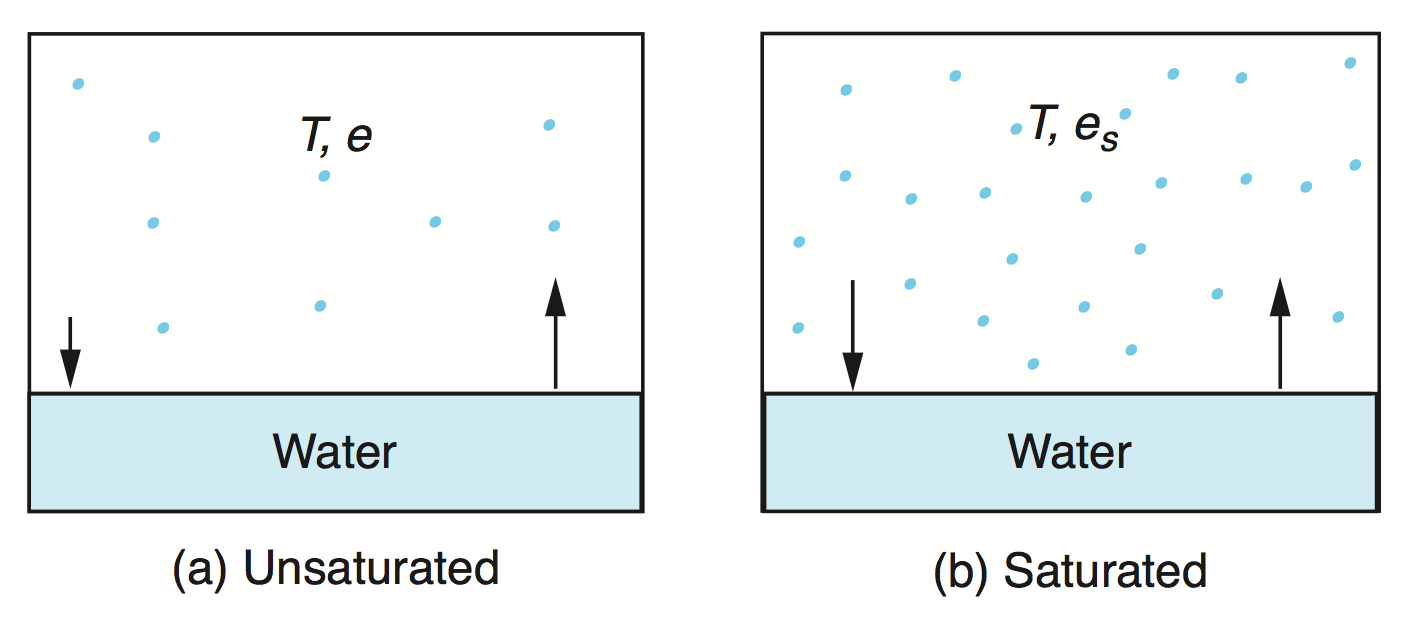
\includegraphics[width=1\textwidth]{fig1}\\
    \centering \small From Wallace and Hobbs (2006)
    \end{minipage}
    \end{column}
    \begin{column}{.5\textwidth}
    \begin{minipage}[c][0.8\textheight][c]{\linewidth}
   \begin{itemize}
   	\item Consider a small closed box whose floor is covered by pure water at temperature $T$
   	\item Let's assume that the air is initially completely dry
   	\item Evaporation begins and the number of water molecules in the box (thus $e$) increases
   	\item As $e$ gets larger, the fast water condense back into liquid form
   \end{itemize}
      \end{minipage}
    \end{column}
  \end{columns}
\end{frame}

%------------------------------------------------

\begin{frame}{Moisture Parameters: Saturation Vapor Pressure}
\begin{columns}[T]
    \begin{column}{.5\textwidth}
    \begin{minipage}[c][0.8\textheight][c]{\linewidth}
    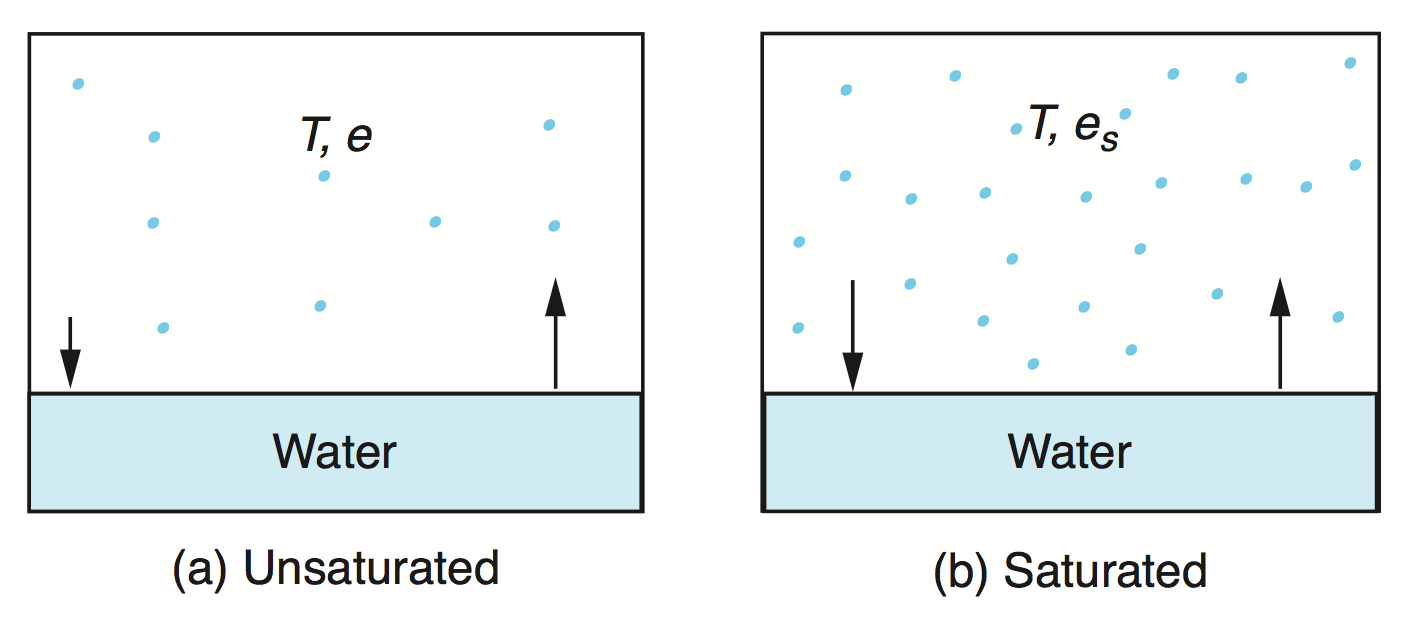
\includegraphics[width=1\textwidth]{fig1}\\
    \centering \small From Wallace and Hobbs (2006)
    \end{minipage}
    \end{column}
    \begin{column}{.5\textwidth}
    \begin{minipage}[c][0.8\textheight][c]{\linewidth}
   \begin{itemize}
   	\item If the rate of condensation $>$ rate of evaporation, then the box is \textbf{unsaturated} at $T$
   	\item If the rate of condensation $=$ rate of evaporation, then the box is \textbf{saturated} at $T$
   	\item The pressure exerted by the water vapor int he box is called the \textbf{saturation vapor pressure $e_s$}
   \end{itemize}
      \end{minipage}
    \end{column}
  \end{columns}
\end{frame}

%------------------------------------------------

\begin{frame}{Moisture Parameters: Saturation Vapor Pressure}
\textbf{Saturation Vapor Pressure Deficit}
\begin{fancydefs}
	The difference between the saturated vapor pressure at a particular temperature and the water vapor pressure
	$$VPD = e_s(T) - e$$
\end{fancydefs}
\begin{itemize}
	\item $VPD$ is sometimes referred to as the ``drying power'' of air in ecology problems
\end{itemize}
\end{frame}

%------------------------------------------------

\begin{frame}{Moisture Parameters: Saturation Vapor Pressure}
\textbf{A quick aside}
\begin{itemize}
	\item You might hear phrases like
	\begin{fancyquotes}
		The air is saturated with water vapor\\
		Warm air holds more wv than cold air\\
		The air cannot hold more wv
	\end{fancyquotes}
	These suggest that air absorbs water vapor like a sponge.\\~\\
	\textbf{Wrong! Stop That!}
\end{itemize}
\end{frame}

%------------------------------------------------

\begin{frame}{Moisture Parameters: Saturation Vapor Pressure}
\textbf{A quick aside}
\begin{itemize}
	\item Recall Dalton's Law of Partial Pressures - the total pressure is equal to the partial pressure of each constituent
	\item Thus, the phase change of water between liquid and vapor form is independent of air
	\item Water vapor that is in equilibrium with water at $T$ should more appropriately called the \textbf{equilibrium vapor pressure}
\end{itemize}
\end{frame}

%------------------------------------------------

\begin{frame}{Moisture Parameters: Saturation Vapor Pressure}
\begin{itemize}
	\item Recall Dalton's Law of Partial Pressures - the total pressure is equal to the partial pressure of each constituent
	\item Thus, the phase change of water between liquid and vapor form is independent of air
	\item Water vapor that is in equilibrium with water at $T$ should more appropriately called the \textbf{equilibrium vapor pressure}
\end{itemize}
\end{frame}

%------------------------------------------------

\begin{frame}{Moisture Parameters: Saturation Vapor Pressure}
\begin{itemize}
	\item How do we find $e_s(T)$? By using the Clausius–Clapeyron equation
	\item It relates the saturation vapor pressure to temperature
	\item From Maxwell's Equations (\nth{2} Law of Thermodynamics)
	$$\frac{de_s}{e_s} = \frac{L_v}{R_v} \frac{dT}{T^2}$$
	where
	\begin{itemize}
		\item $e_s$ is saturation vapor pressure
		\item $L_v$ is the latent heat of vaporization
		\item $T$ is temperature
		\item $R_v$ is the gas constant for water vapor
	\end{itemize}
\end{itemize}
\end{frame}

%------------------------------------------------

\begin{frame}{Moisture Parameters: Saturation Vapor Pressure}
\begin{itemize}
	\item We integrate from state 1 to state 2
	\begin{align*}
		\int^{S2}_{S1}\frac{de_s}{e_s} &= \int^{S2}_{S1}\frac{L_v}{R_v} \frac{dT}{T^2}\\
		\ln\left(\frac{e_s(S2)}{e_s(S1)}\right) &= \frac{L_v}{R_v}\left(\frac{1}{T(S1)} - \frac{1}{T(S2)}\right)\\
		ln\left(\frac{e_s}{e_{s0}}\right) &= \frac{L_v}{R_v}\left(\frac{1}{T_0} - \frac{1}{T}\right)
	\end{align*}
	where we let $S1$ represent a reference state (denoted with  subscript 0)
	\item $T(S1)=T_0=273.1\ \kelvin$
	\item Experimental data has shown $e_s(S1)=e_{s0}=6.11\ \hecto\pascal$
\end{itemize}
\end{frame}

%------------------------------------------------

\begin{frame}{Moisture Parameters: Saturation Vapor Pressure}
\begin{itemize}
	\item Rearranging gives $e_s$ for any $T$
	$$e_s = 6.11\exp \left[ \frac{L_v}{R_v}\left(\frac{1}{273.1} - \frac{1}{T}\right)\right]$$
	\item From this, we can solve for the vapor pressure $e$ from measurements of $RH$ and $T$ by way of
	$$RH=100\frac{e}{e_s}$$
\end{itemize}
\end{frame}

%------------------------------------------------

\begin{frame}{Moisture Parameters: Saturation Vapor Pressure}
\begin{columns}[T]
    \begin{column}{.4\textwidth}
    \begin{minipage}[c][0.7\textheight][c]{\linewidth}
    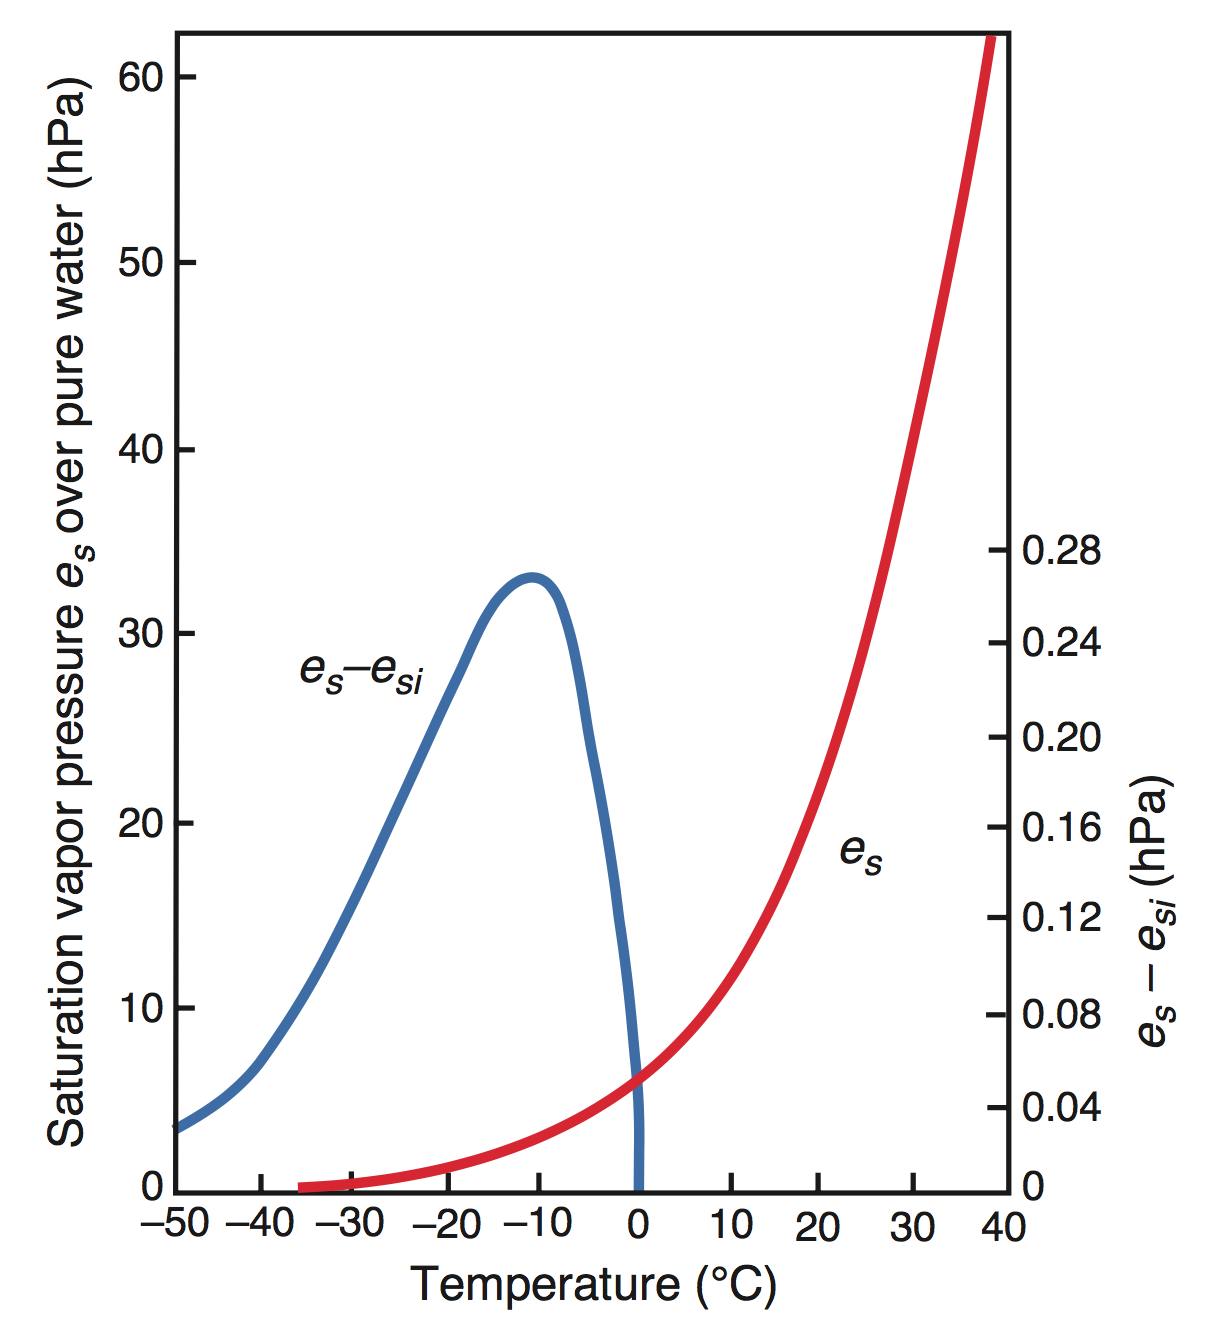
\includegraphics[width=1\textwidth]{fig2}\\
    \centering \small From Wallace and Hobbs (2006)
    \end{minipage}
    \end{column}
    \begin{column}{.6\textwidth}
    \begin{minipage}[c][0.6\textheight][c]{\linewidth}
   \begin{itemize}
   	\item The evaporation rate increases with increasing temperature
   	\item Thus, $e_s$ increase with increasing temperature
   	\item Its magnitude only depends on temperature
   \end{itemize}
      \end{minipage}
    \end{column}
  \end{columns}
\end{frame}

%------------------------------------------------

\begin{frame}{Moisture Parameters: Saturation Mixing Ratio}
\textbf{Saturation Mixing Ratio}
\begin{fancydefs}
	The amount of water vapor in a volume of air that is saturated, expressed as the ratio of the mass of water vapor $m_{vs}$ to the mass of dry air $m_d$
	$$r_s \equiv \frac{m_{vs}}{m_d}$$
\end{fancydefs}
\begin{itemize}
	\item Both water vapor and dry air obey the ideal gas law
	$$r_s = \frac{\rho^\prime_{vs}}{\rho^\prime_{d}} = \cfrac{\cfrac{e_s}{R_vT}}{\cfrac{(p-e_s)}{R_dT}} = \frac{R_d}{R_v}\frac{e_s}{p-e_s}=\epsilon\frac{e_s}{p-e_s}$$
\end{itemize}
\end{frame}

%------------------------------------------------

\begin{frame}{Moisture Parameters: Saturation Mixing Ratio}
\begin{itemize}
	\item Given typical values in the atmosphere, $p\gg e_s$, so
	\begin{align*}
		r_s &=\epsilon\frac{e_s}{p-e_s} \simeq \epsilon\frac{e_s}{p}\\
		\Aboxed{r_s &\simeq 0.622\frac{e_s}{p}}
	\end{align*}
	
\item Thus, $r_s$ is inversely proportional to total pressure at a given temperature
\item Since $e_s$ = $e_s(T)$, then $r_s$ = $r_s(p,T)$
\item This can be seen on a skew T-$\ln$ p chart
\end{itemize}
\end{frame}

%------------------------------------------------

\begin{frame}{Moisture Parameters: Saturation Mixing Ratio}
\begin{columns}[T]
    \begin{column}{.68\textwidth}
    \begin{minipage}[c][0.9\textheight][c]{\linewidth}
    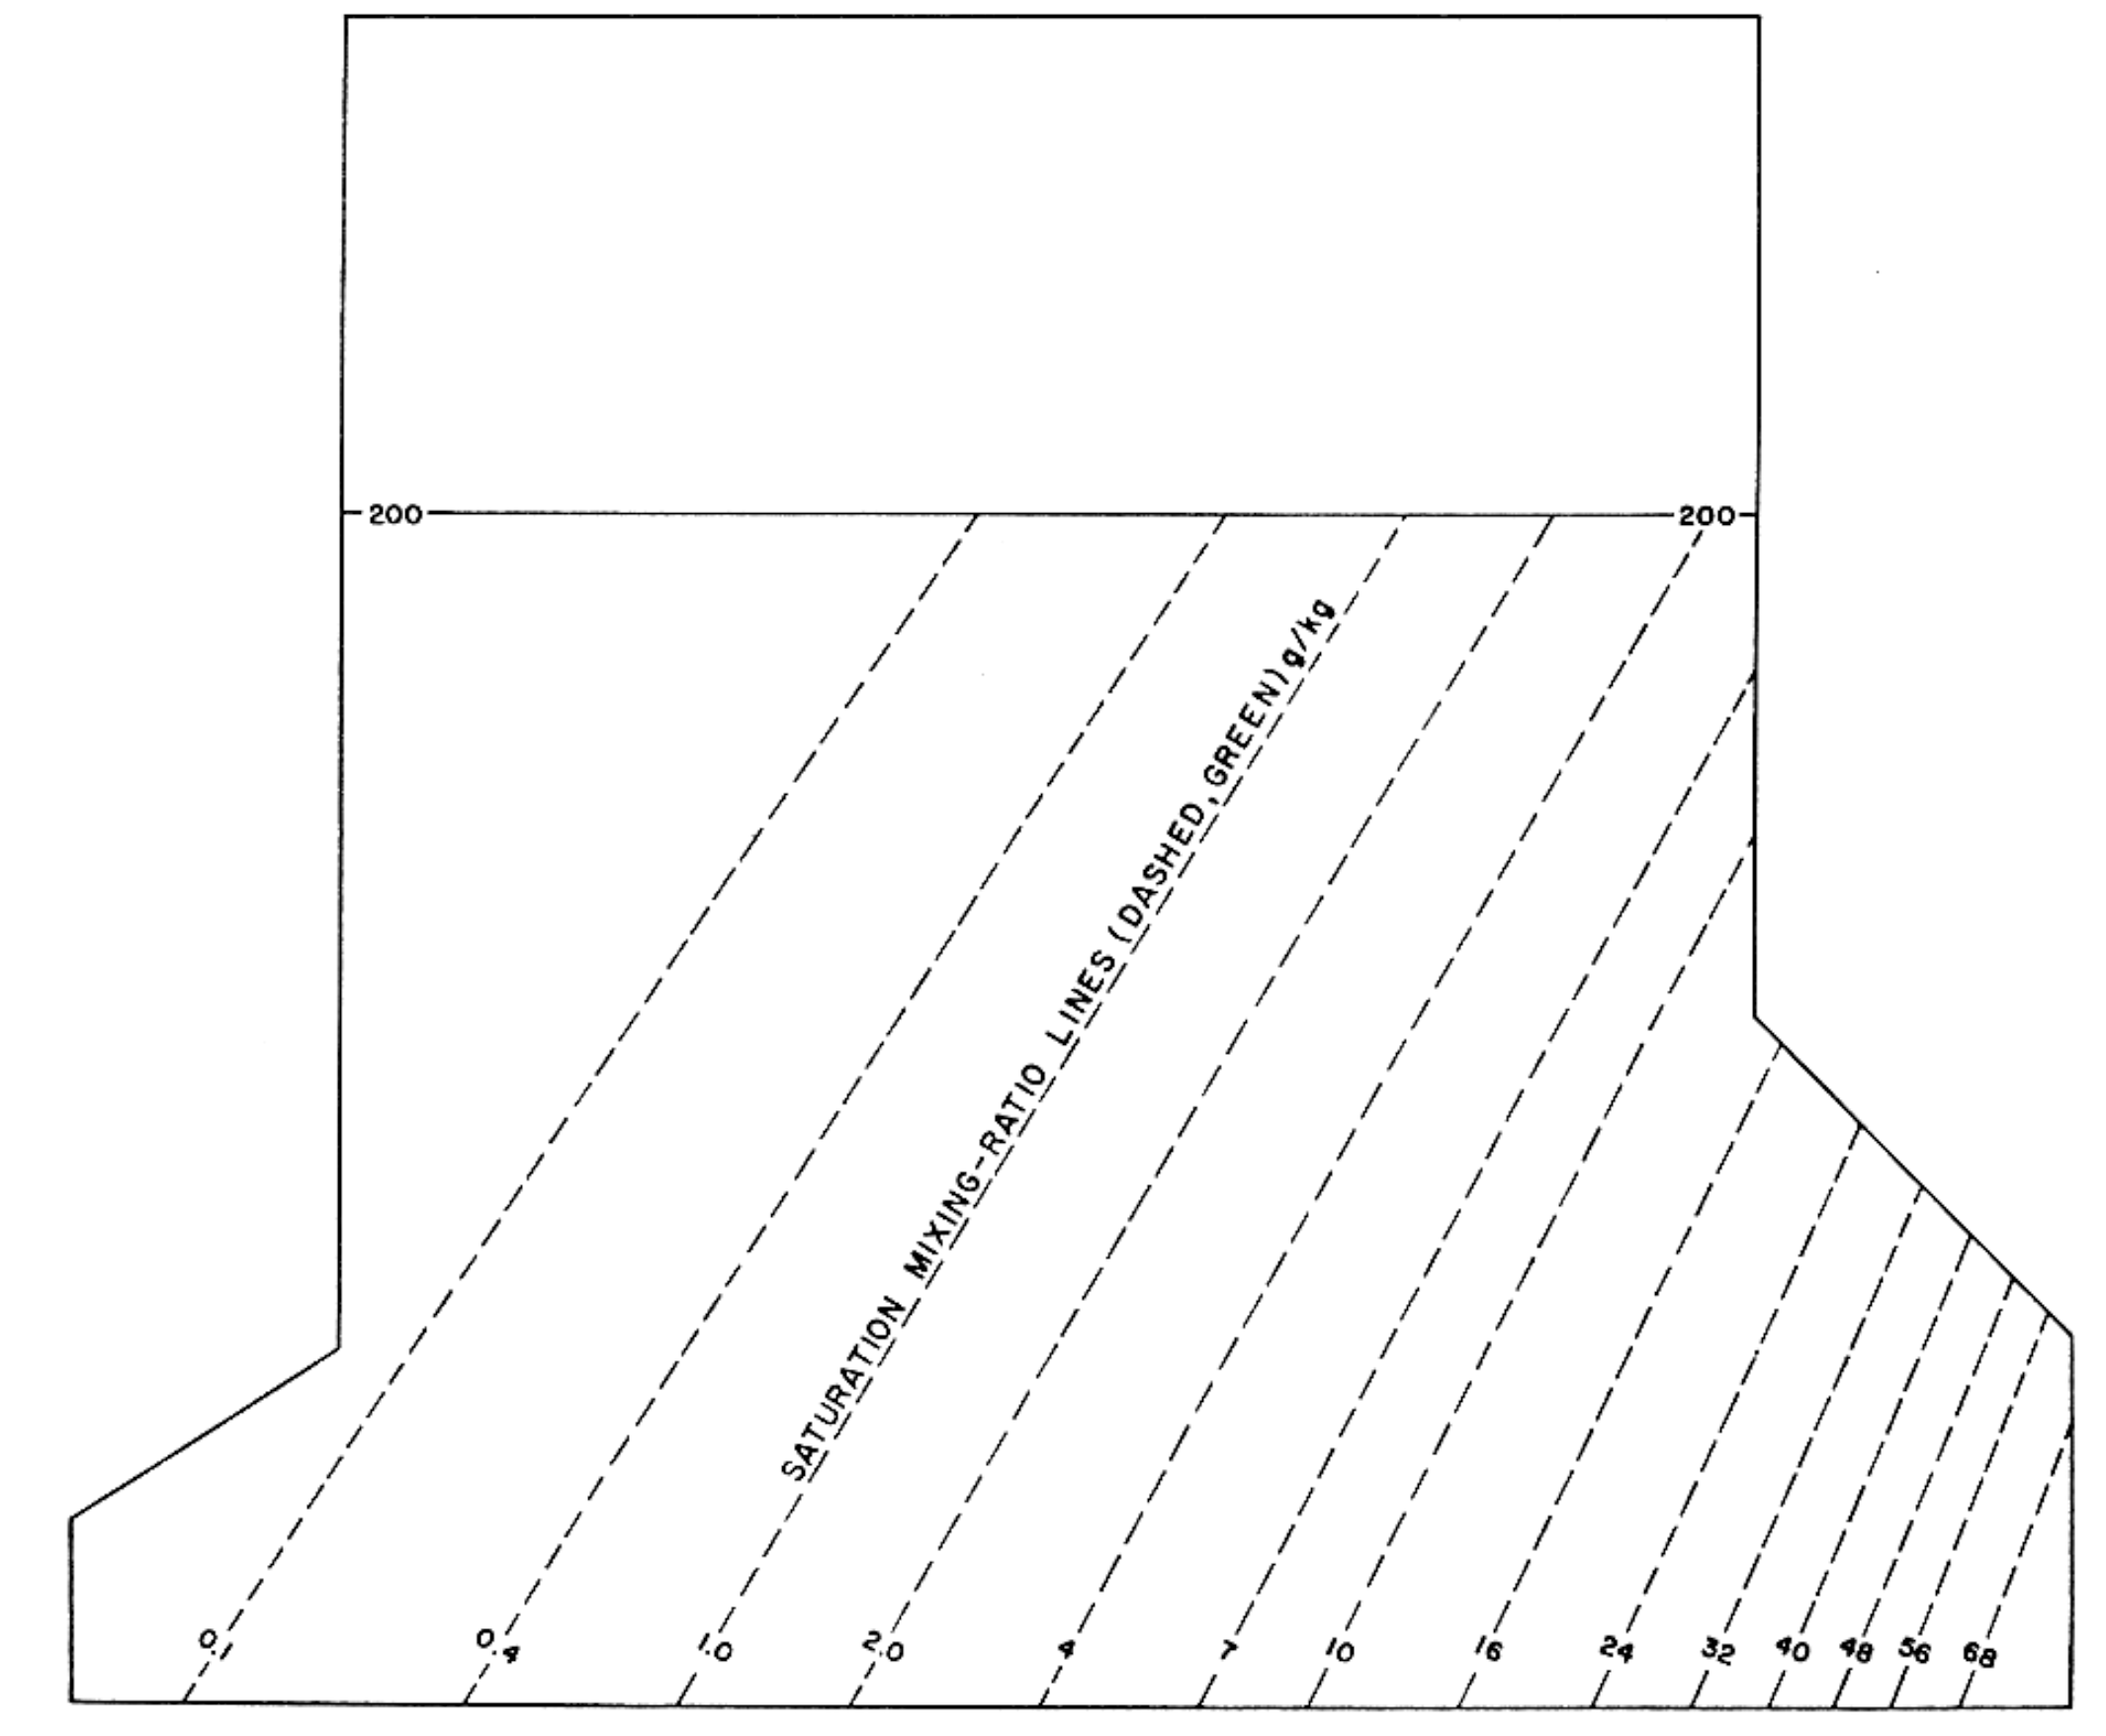
\includegraphics[width=1\textwidth]{fig3}\\
    \end{minipage}
    \end{column}
    \begin{column}{.32\textwidth}
    \begin{minipage}[c][0.8\textheight][c]{\linewidth}
   \begin{itemize}
   	\item For constant $T$, $r_s$ increases with decreasing $p$
   	\item For constant $p$, $r_s$ increases with increasing $T$
   \end{itemize}
      \end{minipage}
    \end{column}
  \end{columns}
\end{frame}

%------------------------------------------------

\begin{frame}{Moisture Parameters: Relative Humidity and Dew Point}
\textbf{Relative Humidity}
\begin{fancydefs}
	The ratio of the mixing ratio to the saturation mixing ratio at the same temperature and pressure
	$$RH \equiv 100\frac{r}{r_s}\simeq100\frac{q}{q_s}\simeq100\frac{e}{e_s}$$
\end{fancydefs}
~\\
\textbf{Dew Point Temperature}
\begin{fancydefs}
	The temperature to which air must be cooled at constant pressure for it become saturated w.r.t water
	$$T_d = T(r_s = r)$$
	$$T_d \simeq T-\frac{100-RH}{5}$$
\end{fancydefs}
\end{frame}

%------------------------------------------------

\begin{frame}{Moisture Parameters: Lifting Condensation Level}
\textbf{Lifting Condensation Level (LCL)}
\begin{fancydefs}
	The level to which a moist unsaturated air parcel can be lifted adiabatically before becoming saturated
\end{fancydefs}
\begin{itemize}
	\item As the parcel rises, $r$ and $\theta$ remain constant while $r_s$ decreases until it equals $r$ (at the LCL)
	\item The LCL is located where dry adiabat and $r_s$ line intersect
	\begin{figure}
		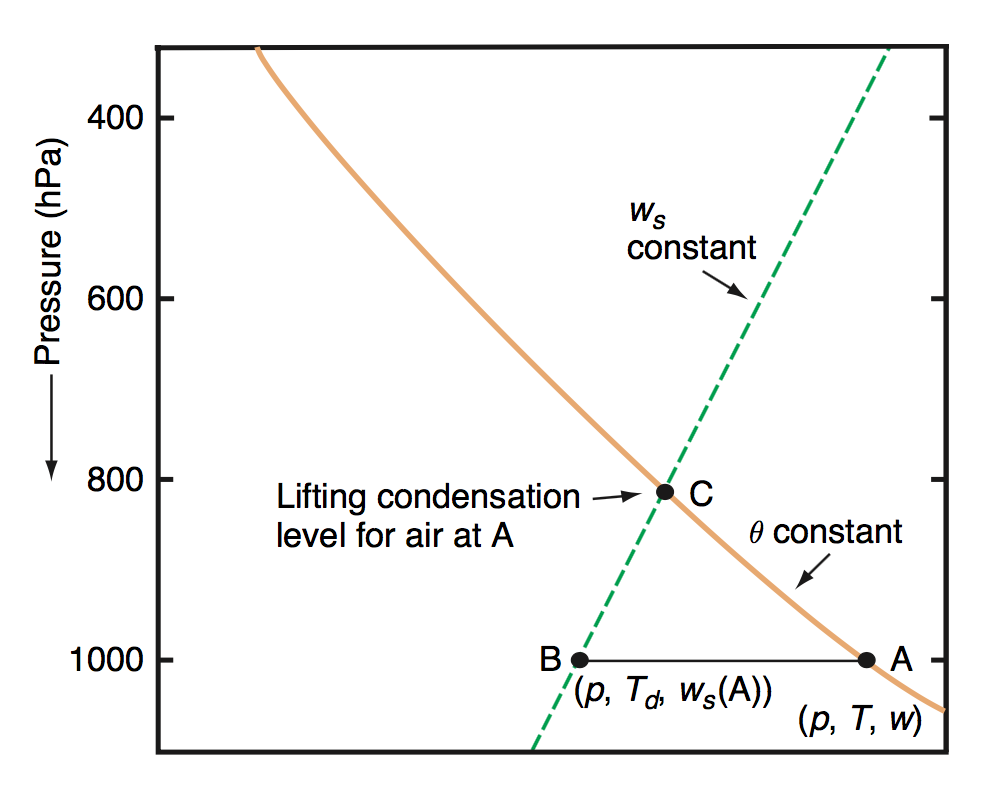
\includegraphics[width=0.5\textwidth]{fig4}
	\end{figure}
\end{itemize}
\end{frame}

%------------------------------------------------
\subsection{Saturated Adiabatic Processes}
\begin{frame}{Saturated Adiabatic Processes}
\begin{itemize}
	\item When an air parcel rises in the atmosphere, $T$ decreases with increasing height until it becomes saturated
	\item Condensation of liquid water occurs as the parcel is lifted further, which releases latent heat
	\item Thus, the lapse rate of the rising parcel is reduced 
	\end{itemize}
\end{frame}

%------------------------------------------------

\begin{frame}{Saturated Adiabatic Processes}
\begin{itemize}
	\item If all the condensation remains in the air parcel, the process is considered reversible and thus adiabatic
	\item Although latent heat is released, as long as it remains within the confines of the air parcel then the parcel underwent a \textbf{saturated adiabatic process}
	\item If the condensation falls out of the parcel then the process is irreversible because condensation carries heat - so not really adiabatic
	\item In this case, it is called a \textbf{pseudoadiabatic process} (in practice the saturated adiabatic and pseudoadiabtic lapse rates are approximately the same)
	\end{itemize}
\end{frame}
%------------------------------------------------
\begin{frame}{Saturated Adiabatic Lapse Rate}
\begin{itemize}
	\item We won't derive this in class, but for posterity here is the saturated adiabatic lapse rate
	$$\Gamma_s \simeq \frac{\Gamma_d}{1+\cfrac{L_v}{c_p}\left(\cfrac{\partial r_s}{dT}\right)_p}$$
	\item Note that the denominator is $>1$, so $\Gamma_d > \Gamma_s$, which agrees with our expectation
	\item Values range from $4\ \kelvin\ \kilo\reciprocal\gram$ near the ground in warm moist air to $6$-$7\ \kelvin\ \kilo\reciprocal\gram$ in the middle portion of the troposphere
\end{itemize}
\end{frame}
%------------------------------------------------
\begin{frame}{Saturated Adiabatic Lapse Rate}
\begin{itemize}
	\item We won't derive this in class, but for posterity here is the equivalent potential temperature $\theta_e$
	\item Just as dry adiabats are lines of constant $\theta$, moist adiabats are lines of constant $\theta_e$
	$$\theta_e \simeq \theta \exp\left(\frac{L_v r_s}{c_pT}\right)$$
\end{itemize}
\end{frame}

%------------------------------------------------
\begin{frame}{Saturated Adiabatic Processes}
\begin{figure}
	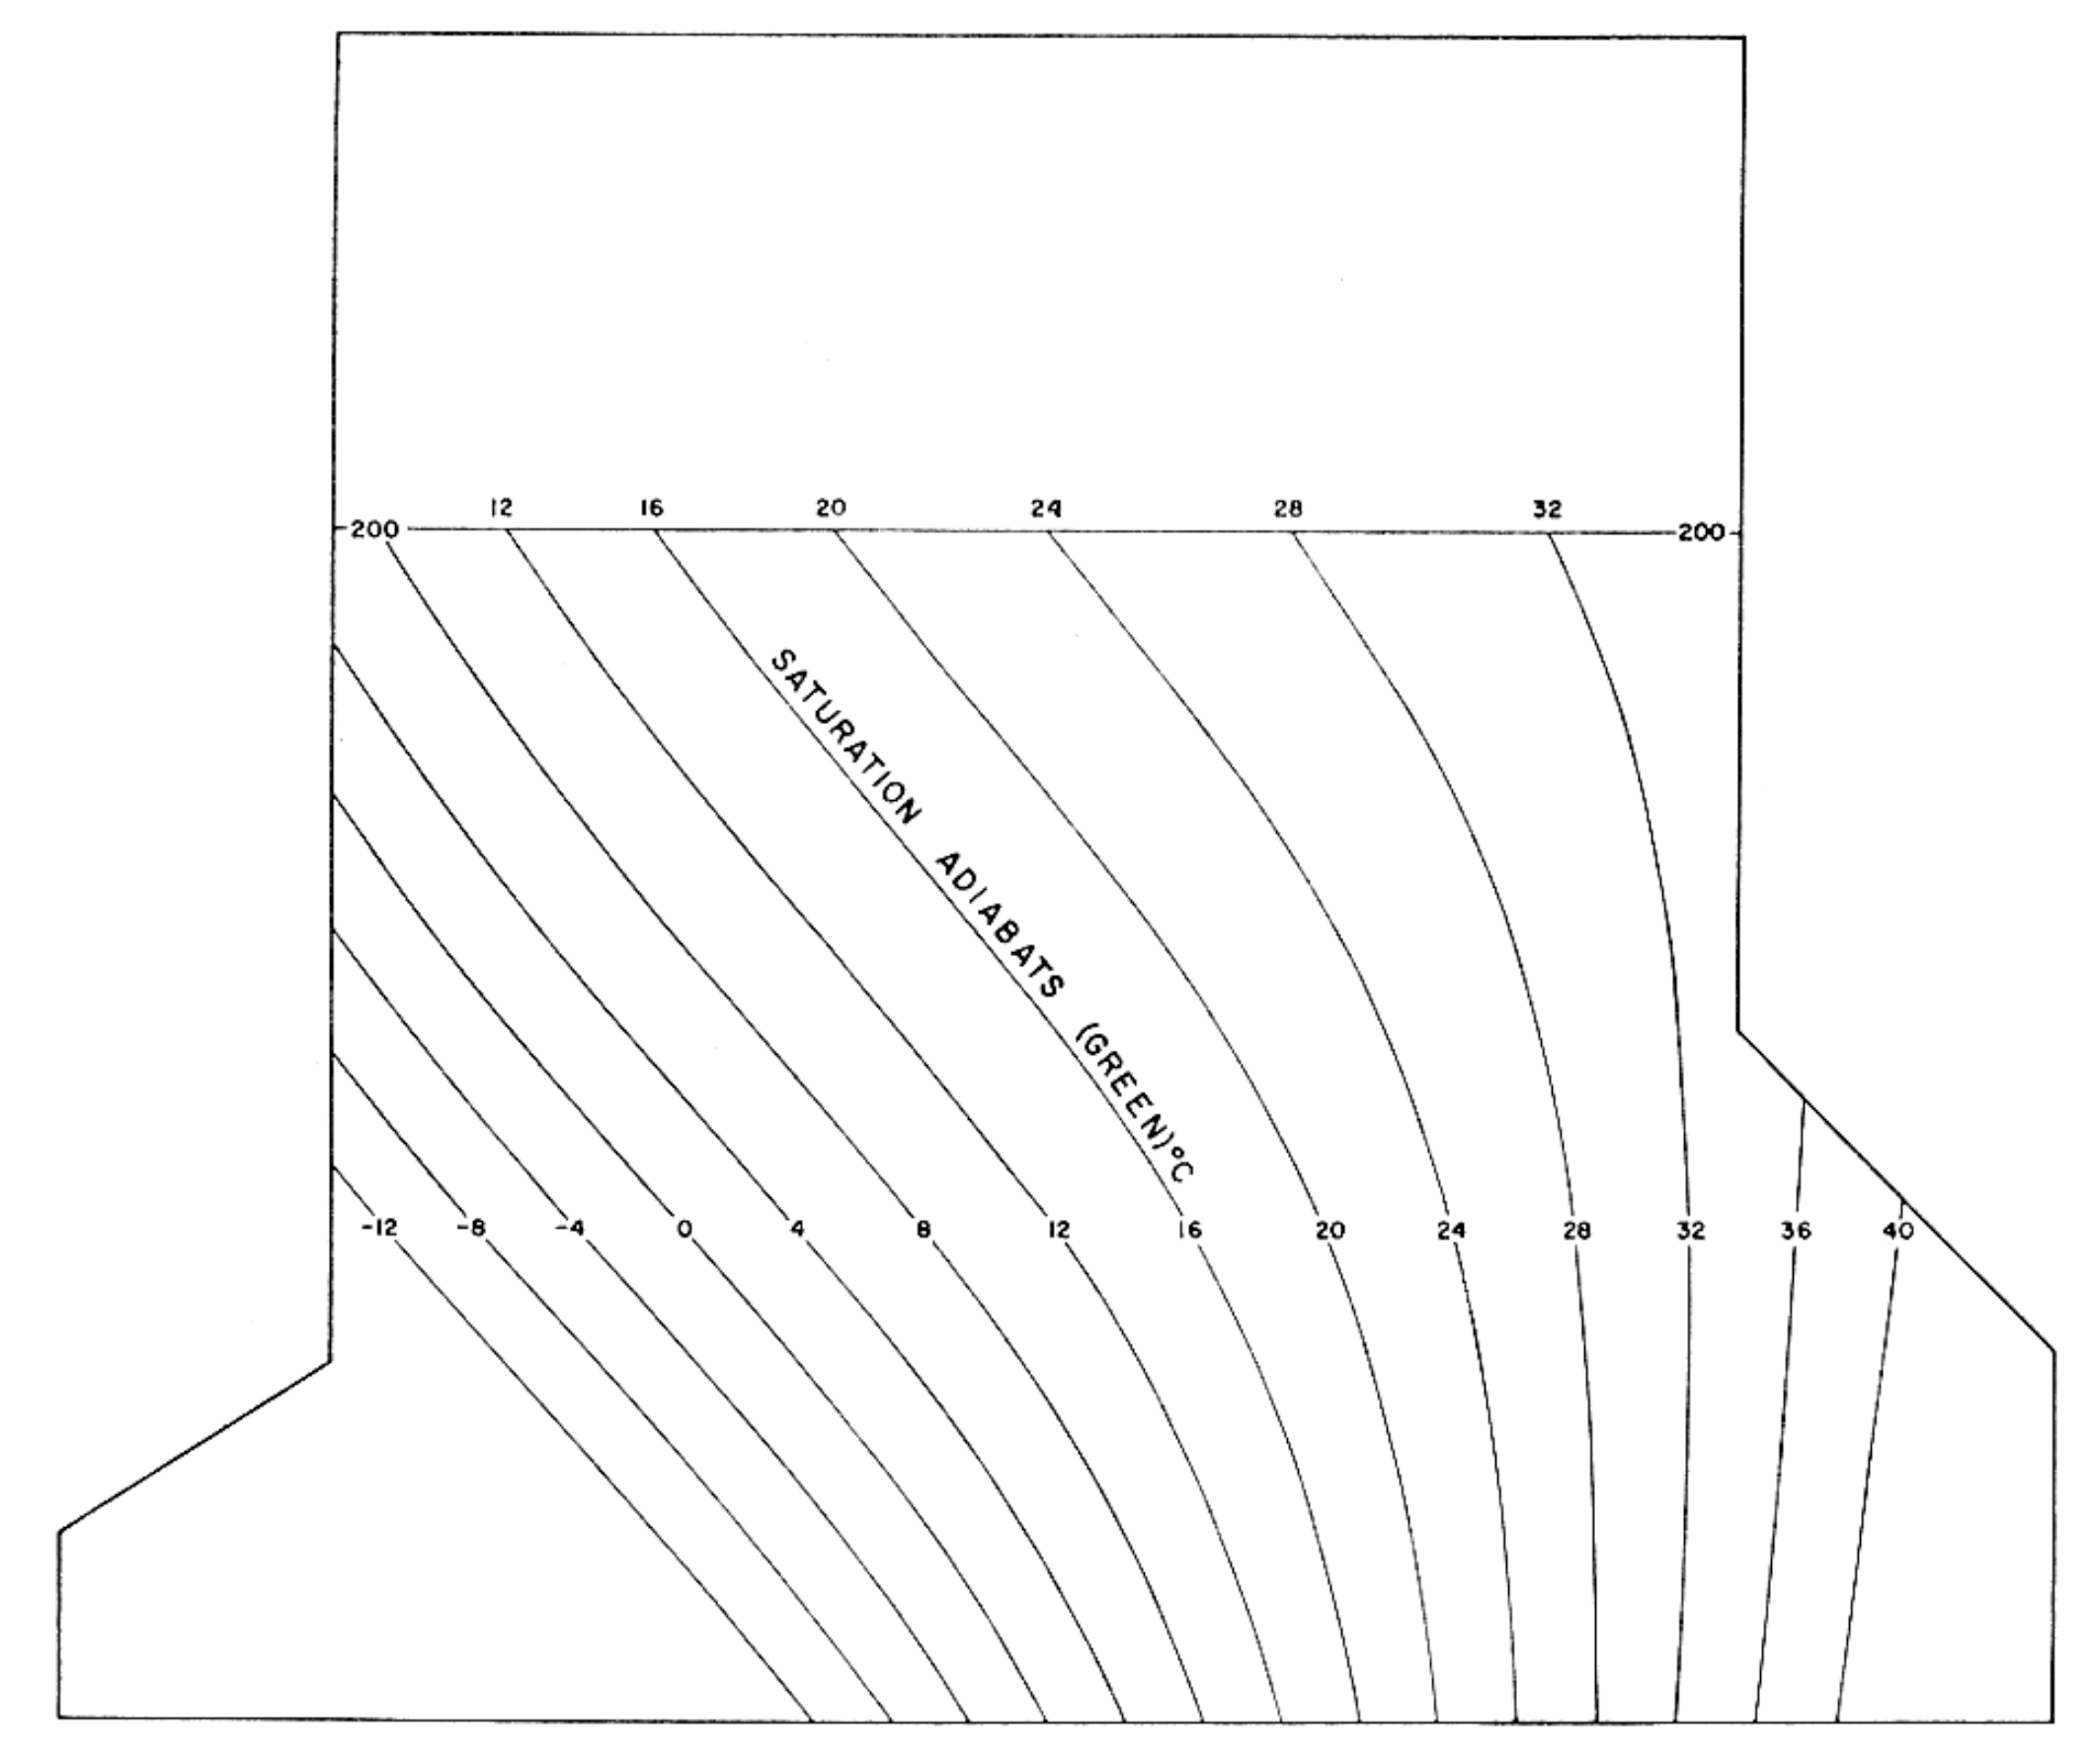
\includegraphics[width=0.9\textwidth]{fig5}
\end{figure}
\end{frame}


%------------------------------------------------



\end{document}

